\setlength{\footskip}{8mm}

\chapter{Methodology}
\label{ch:methodology}

\textit{This chapter focuses on the system architecture and the different mechanisms for communication. The reasons behind the choice of these particular methods are also put forward. Finally, the experimental design is detailed in preparation for Chapter \ref{ch:results}.
}

\section{System Overview}\label{sect:sysov}
The main goal of the system that was developed in this study is to facilitate communication between a web application and a remote drone. This is accomplished with the use of SSH port forwarding and a remote-procedure-call framework called Apache Thrift.

The overall operation is as follows:
\begin{enumerate}
  \item Forward Raspberry Pi port to web server using reverse tunnel.
  \item Run Apache Thrift server on Raspberry Pi.
  \item Execute client scripts that call functions on Thrift server through the SSH tunnel. The server in turn sends MAVLink commands to the local Pixhawk.
\end{enumerate}

As shown in Figure \ref{fig:system}, the drone communicates with the web application through the use of a reverse SSH tunnel. The web app is then be able to communicate with the Pi as if it were on a local port. In the next step, the web app executes client scripts with the mission parameters from the web server. These scripts call functions on the Thrift server running on the Raspberry Pi through the port tunnelled from the Pi. A more comprehensive description can be found in Section \ref{sect:communicationlayer}.

The server is connected to the Pixhawk through the Dronekit API, a high-level MAVLink API written in Python. Dronekit provides many wrapper functions and objects that make communication with the Pixhawk more accessible. The fact that the Thrift server is also running in Python, makes combining these two frameworks a simple matter. Further details can be found in Section \ref{sect:commandlayer}.

\begin{figure}[t]
	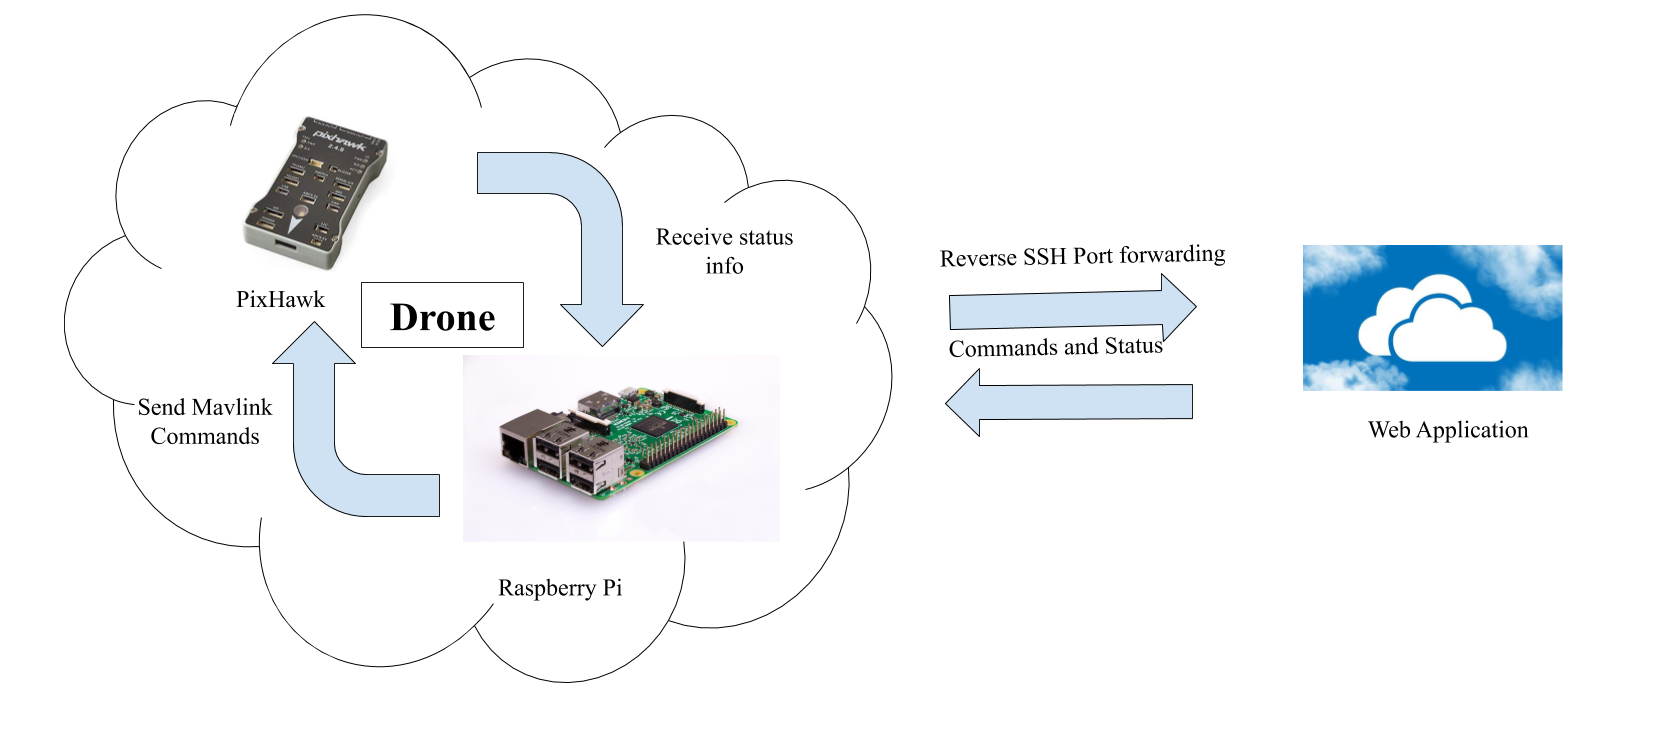
\includegraphics[width=\textwidth]{Ch3/Drone_Architecture}
	\caption{Basic system architecture.}
	\label{fig:system}
\end{figure}
\FloatBarrier

The operation of the system developed in this study can be divided into two layers: communication and command (see Figure \ref{fig:layersystem}). The communication layer handles the exchange of information between the web app and the Raspberry Pi (which acts as an intermediary between the web application and the Pixhawk). This is done over the Internet with the Raspberry Pi using a 4G USB LTE dongle to communicate with the web server. On the other hand, the command layer handles the mission uploading, execution and status retrieval using the MAVLink Dronekit API. 

\begin{figure}[t]
	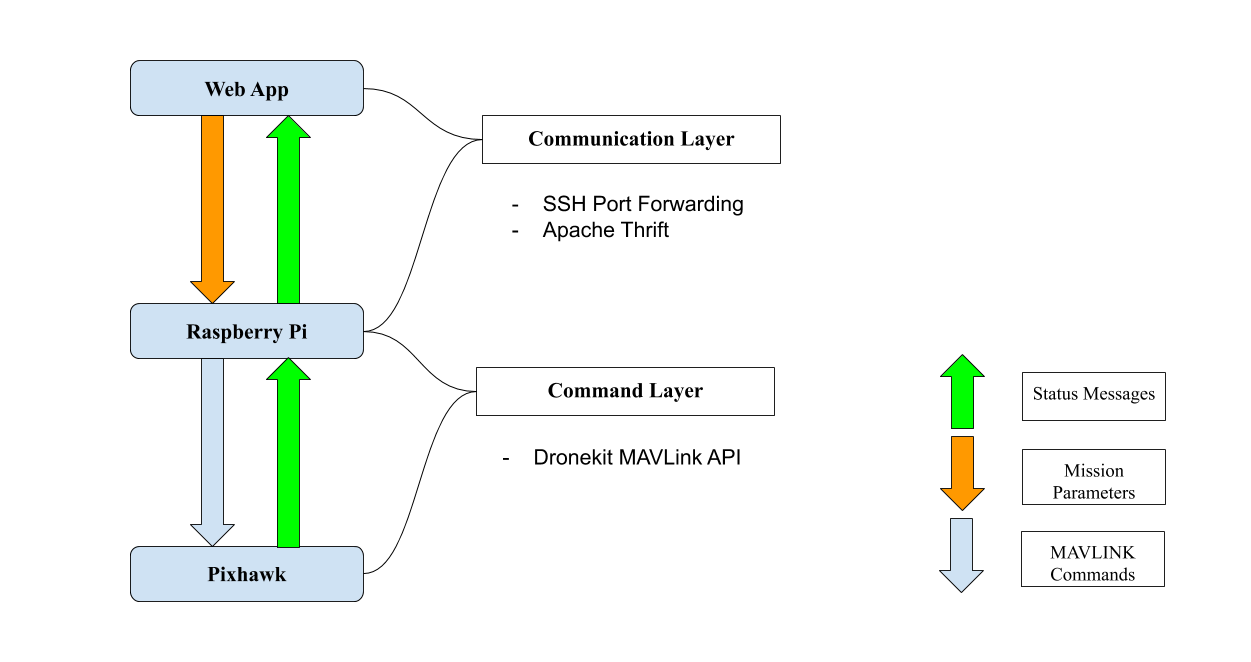
\includegraphics[width=\textwidth]{figures/Ch3/Layer_Drone_Architecture.png}
	\caption{Two-Layer system architecture.}
	\label{fig:layersystem}
\end{figure}
\FloatBarrier

Once again, it is stressed that the application is the one sending commands instead of the user himself/herself. Under normal conditions, the user would have to SSH to the Pi and then execute commands there.

\begin{table}[t]
 \caption{Technologies used in the development of the system.}
 \linespread{0.8}\selectfont
 \begin{center}
     \begin{tabular}{|m{5cm}|m{8cm}|} 
     \hline
     \textbf{Communication Layer} & SSH (Port forwarding), Apache Thrift \\ 
     \hline
     \textbf{Command Layer} & Dronekit MAVLink API (Python), Apache Thrift (Python) \\ 
     [1ex] 
     \hline
 \end{tabular}
 \end{center}{}
\end{table}
\FloatBarrier

Although the web application is considered as a GCS, the Thrift server running on the Raspberry Pi is actually more similar to a GCS and hence should be called one.

Furthermore, there are two main types of messages or communication that are transferred between a drone and the application. The first type of message contain information about the status of the drone. These are sent from the drone to the web application. The second type contains commands sent from the web application to the drone and mainly involves mission parameters from the user.


% There are two layers to the operation of this system. The first layer involves using SSH to forward a port on the webserver onto the onboard computer on the drone. The second layer consists of the command aspect. A server running on the Raspberry Pi sends commands to the Pixhawk flight controller.

% Each type and its complementary communication mechanism is explained further in its own section, i.e. sections \ref{sect:dronereporting} and \ref{sect:dronec&c}, respectively. 

% There are two stages to the operation of this system. The first stage involves using SSH to access the onboard computer on the drone. Scripts that send Mavlink commands to the Pixhawk are then executed. More detail can be found in Section \ref{sect:dronec&c}.

\section{Communication Layer}\label{sect:communicationlayer}
Under normal circumstances, the on-board computer on the drone can be accessed using SSH and Dronekit scripts can then be execute to invoke commands on the Pixhawk. 

However, in the web application\textquotesingle s case, the user is going to send mission parameters from the web app instead to the on-board computer. The web application executes client Thrift scripts that call functions on the remote Thrift server. Furthermore, the more detailed commands, such as takeoff and flight control, are abstracted away from the user. He or she only needs to specify the core mission parameters, such as destination coordinates, maximum altitude, etc.

\subsection{Connection Nature}
Since the drone is connected to the Internet through a USB LTE dongle using a SIM card, this creates a problem. The SIM card sits behind its provider\textquotesingle s NAT (network address translation service). Since the NAT only exposes one public IP address to the Internet, there is no simple way of knowing the SIM\textquotesingle s (the drone\textquotesingle s) IP address. This makes the standard client-server architecture useless. Figure \ref{fig:nat} shows an example of NAT in action.

\begin{figure}[t]
	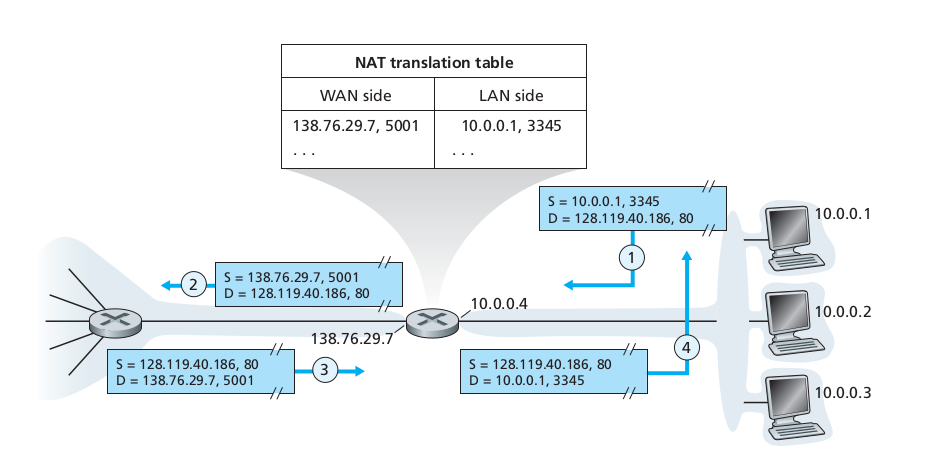
\includegraphics[width=\textwidth]{Ch3/nat}
	\caption{Network address translation. Reprinted from \protect\citeA{cn}.}
	\label{fig:nat}
\end{figure}
\FloatBarrier

\subsection{Reverse SSH Tunnelling}\label{subsect:ssh}
To combat this IP problem, a reverse SSH tunnel is used. This method is also called reverse SSH port forwarding and is simple as well as secure. Basically, a specified port number on the remote machine (in this case, the drone) is “forwarded” to the client (the web application) using another port number. The remote opens an SSH connection to the outside world and specifies that the entry point for this connection is the destination of the remote, i.e. the client.

\begin{figure}[t]
	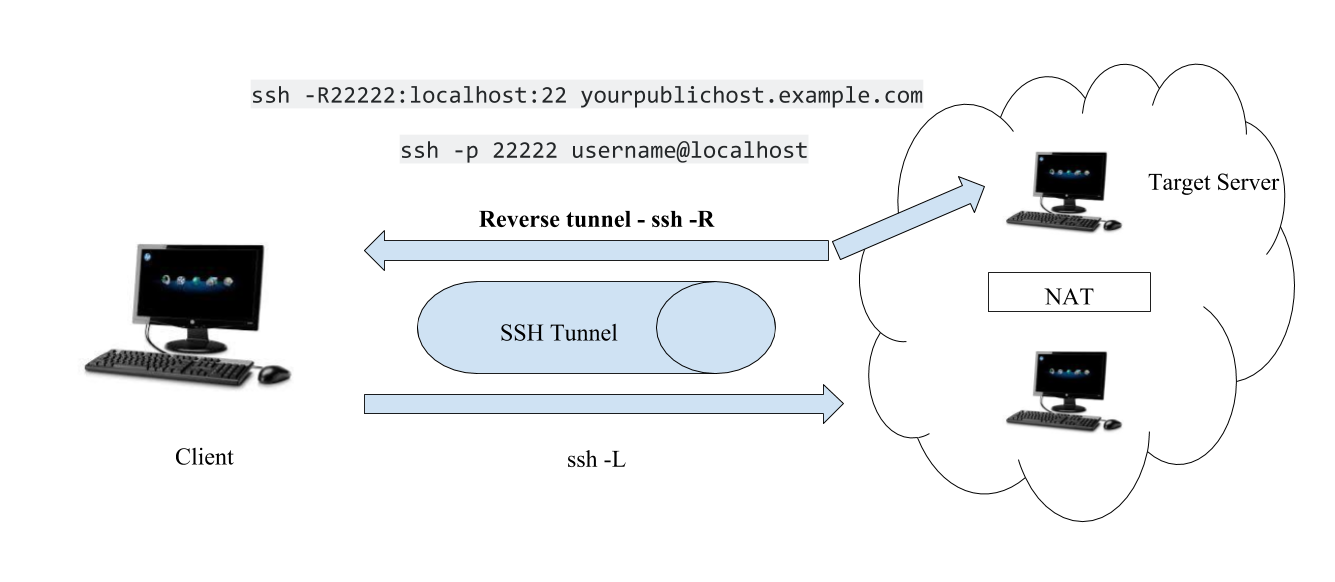
\includegraphics[width=\textwidth]{figures/Ch3/Reverse_Basic.png}
	\caption{Reverse SSH Tunnelling in action.}
	\label{fig:reverse_ssh_basic}
\end{figure}
\FloatBarrier

For example, in Figure \ref{fig:reverse_ssh_basic} above, the target server resides behind a NAT and hence must be the one to open the SSH connection. Anything that attaches to port 22222 on the far end of the tunnel will actually reach "localhost port 22" on the SSH client.

The actual implementation is shown in Figure \ref{fig:reverse_ssh}:

\begin{figure}[t]
	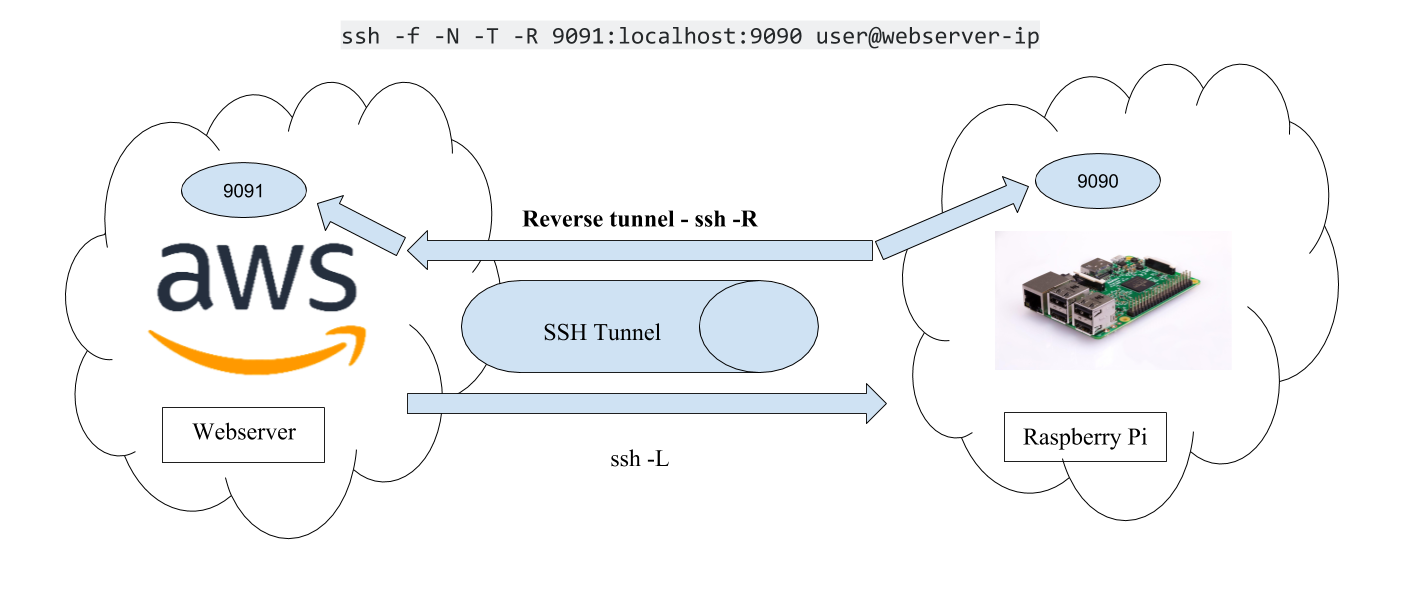
\includegraphics[width=\textwidth]{figures/Ch3/Reverse_SSH.png}
	\caption{Implementation of reverse SSH tunnelling.}
	\label{fig:reverse_ssh}
\end{figure}
\FloatBarrier

When the command shown at the top of Figure \ref{fig:reverse_ssh} is run, all traffic to port 9091 on the web server is directed through an SSH tunnel to port 9090 on the Raspberry Pi, on which the Apache Thrift server is listening. The arguments are defined as:

\begin{itemize}
  \item -f: tells SSH to run as a background daemon
  \item -N: saves system resources if remote execution is not required
  \item -T: disables pseudo-tty allocation for non-interactive sessions
\end{itemize}

\subsection{Apache Thrift}
Now that a tunnel has been established between the web server and the Raspberry Pi, a suitable mechanism is needed in order to facilitate communication between them. Apache Thrift was chosen due to its accessibility, flexibility and scalability. Thrift is an RPC framework that was initially developed at Facebook but has since been open-sourced.

The core functionality of Thrift is defining services and so-called ``structs'' that will be utilized by all clients and servers over the distributed system. This is done in a Thrift file.

Some examples of Thrift services are shown below:
\begin{verbatim}
    void land(),
    void add_delivery_mission(1:double latitude, 2:double longitude, 
        3:double altitude),
    bool report_status(1:i32 drone_id),
\end{verbatim}

% \begin{itemize}
%   \item \texttt{void land()}
%   \item \texttt{void add\_delivery\_mission(1:double latitude, 2:double longitude, 3:double altitude)}
%   \item \texttt{bool report\_status(1:i32 drone\_id)}
% \end{itemize}

% \begin{figure}[h]
% 	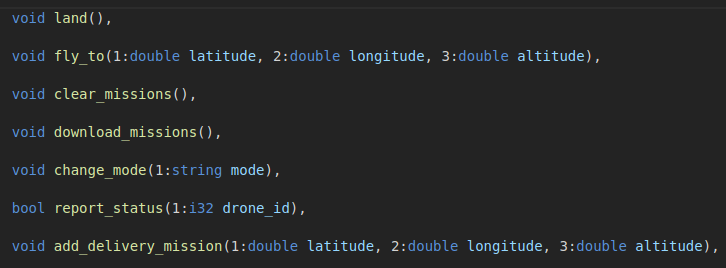
\includegraphics[width=\textwidth]{figures/Ch3/drone_thrift_sample.png}
% 	\caption{Some examples of services defined in Thrift.}
% 	\label{fig:thrift_service}
% \end{figure}
% \FloatBarrier

\newpage
An example of a Thrift struct is shown below:
\begin{verbatim}
    struct Coordinate {
        1: double latitude,
        2: double longitude,
        3: double altitude,
    }
\end{verbatim}[]

% \begin{figure}[h]
% 	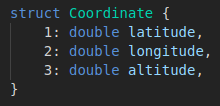
\includegraphics[width=\textwidth]{figures/Ch3/thrift_struct.png}
% 	\caption{Thrift Coordinate struct.}
% 	\label{fig:thrift_struct}
% \end{figure}
% \FloatBarrier

In the example shown above, the \texttt{Coordinate} struct is generated as a Python object ready for use by both the server and client. This struct is used to send coordinate/waypoint information between the client and the server, especially in the farm missions since these usually involve multiple coordinates.

The defined services and structs are used to generate into source code that are then utilized by the Thrift server and client scripts. In this study, this is done in the development environment and committed into the repository so that the production environment, i.e. the Raspberry Pi, already has access to the generated code. The generation is carried out with the following command:

\begin{itemize}
  \item \texttt{thrift --gen <language> <Thrift filename>}
\end{itemize}

As can be seen above, the file can be transformed into any language desired, meaning near limitless cross-platform possibilities. 

\begin{table}[t]
 \caption{Languages supported by Apache Thrift.}
 \linespread{0.7}\selectfont
 \begin{center}
     \begin{tabular}{|m{5cm}|m{8cm}|} 
     \hline
     \textbf{Languages} & ActionScript, C, C++, C\#, Cappuccino, Cocoa, Delphi, Erlang, Go, Haskell, Java, Node.js, Objective-C, OCaml, Perl, PHP, Python, Ruby, Rust, Smalltalk and Swift \\ 
     [1ex] 
     \hline
 \end{tabular}
 \end{center}{}
 \label{table:thriftlang}
\end{table}
\FloatBarrier

All of the languages supported by Thrift are given in Table \ref{table:thriftlang}. The generated code also uses a protocol and a transport type for service. There are several types of protocols, including both binary and text protocols. For this study, a simple binary protocol and a buffered transport is used.

\subsubsection{Thrift Server}
As already stated in Section \ref{sect:sysov}, the Apache Thrift server is run on the Raspberry Pi. Using the SSH tunnel created in Section \ref{subsect:ssh}, the client scripts are able to call functions on this server. The server contains various functions that have been defined as available services in the Thrift file.

The server is connected to the Pixhawk through the Dronekit API and is responsible for controlling the takeoff, landing, mission parameter adding (coordinates and altitude), status reporting and returning to base. This command aspect is further elaborated on in Section \ref{sect:commandlayer}.

There are several different types of servers available in Apache Thrift, as shown in Table \ref{table:thriftservertypes}. For this study, a simple \texttt{TServer} implementation is used.

\begin{table}[t]
 \caption{Server Types supported by Apache Thrift.}
 \linespread{0.7}\selectfont
 \begin{center}
     \begin{tabular}{|m{5cm}|m{8cm}|} 
     \hline
     \textbf{Server Types} & \textbf{Description}\\ 
     \hline
     TSimpleServer & Simple single-threaded blocking server\\
     \hline
     TThreadedServer & Multi-threaded blocking server that allocates a thread to each connection\\
     \hline
     TNonblockingServer & Multi-threaded non-blocking server\\
     \hline
 \end{tabular}
 \end{center}{}
 \label{table:thriftservertypes}
\end{table}
\FloatBarrier

The complete workflow for both Thrift server and client is shown in Figure \ref{fig:thrift_workflow}. It is reminded that the client can only be started after the server has completed setting up the connection to the Pixhawk. Further details on what happens after mission launch can be found in Section \ref{sect:commandlayer} (see Figure \ref{fig:commandworkflow}).

\begin{figure}[t]
	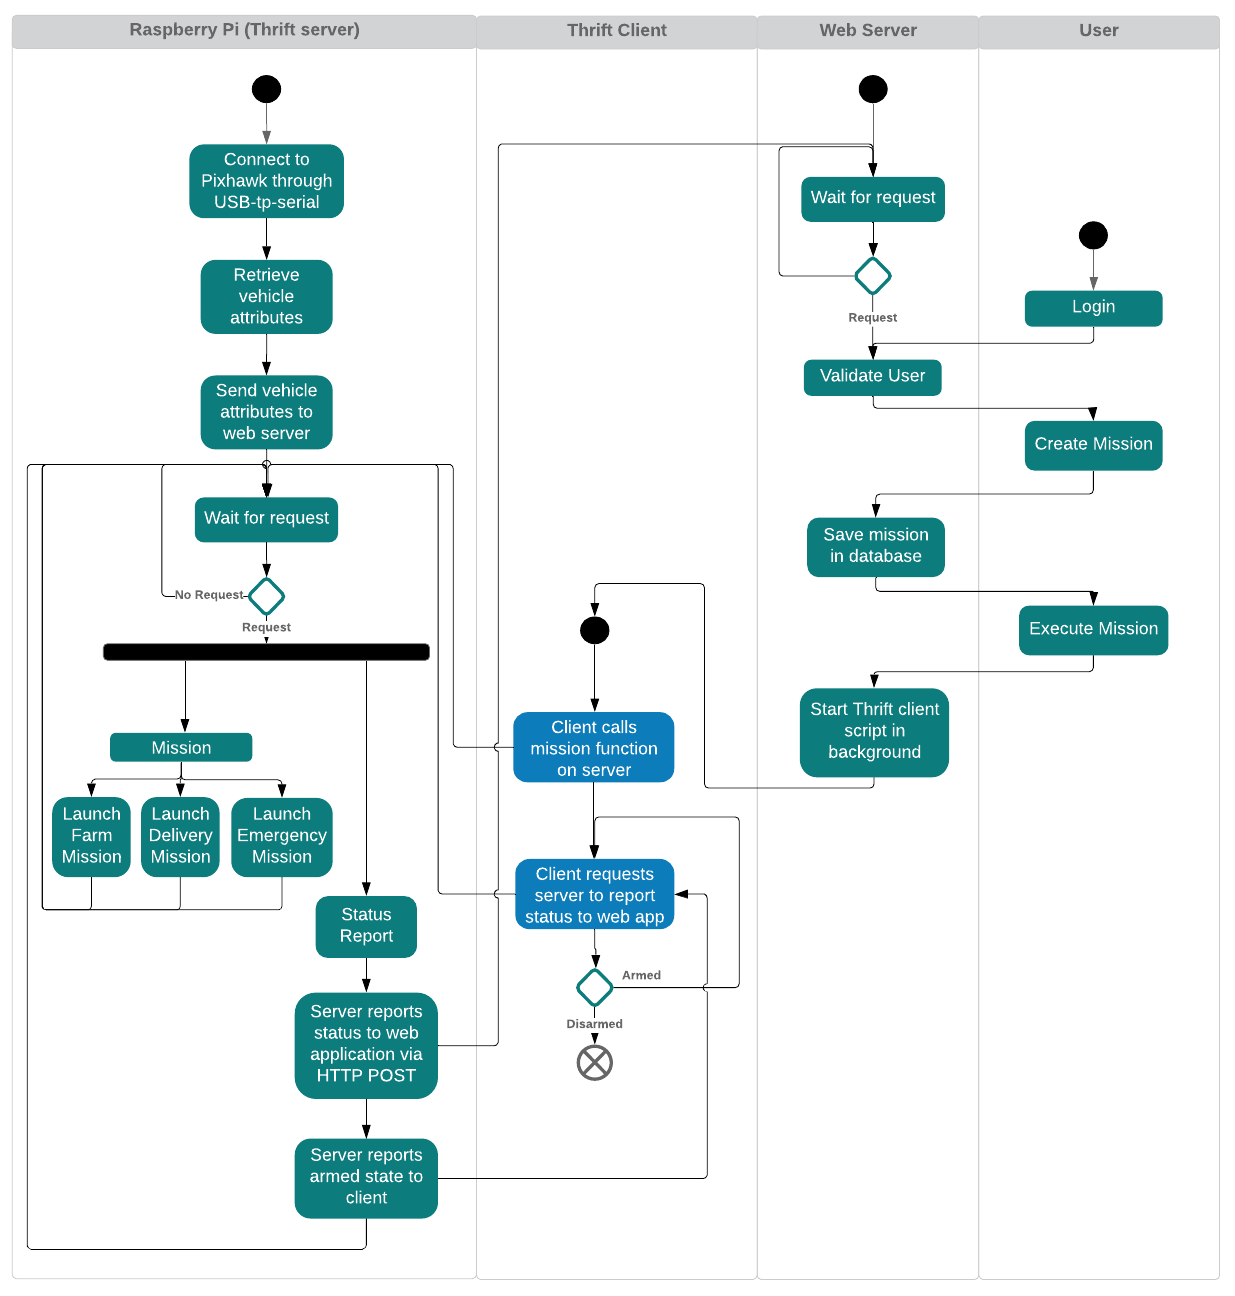
\includegraphics[width=\textwidth, height=21cm]{figures/Ch3/Apache_Thrift_Server.png}
	\caption{Apache Thrift client-server workflow diagram.}
	\label{fig:thrift_workflow}
\end{figure}
\FloatBarrier

\subsubsection{Thrift Clients}
The Thrift clients also utilize the source code generated with the Thrift definition file. The client scripts simply open a socket to the port on which the server is listening on and call functions on the server. There is a separate client script for each mission type, i.e. delivery and farm missions. 

The client scripts are executed as a process in a controller set up by the web application. Once a user clicks on the ``execute'' button, the corresponding controller spawns a process for the Python script and then detaches it from the web application. This means that the Thrift clients are completely asynchronous from the web application and ``fire-and-forget'', only relying on HTTP for feedback to it (see Section \ref{subsect:flightstatus}). 

However, the clients do listen for feedback from the Thrift server on the Raspberry Pi, specifically the drone\textquotesingle s armed status. This is achieved via a return value for the Thrift service for the status check function. As long as the drone remains armed (implying that it is on a mission), the client running on the web server requests the Thrift server on the Pi to send a HTTP POST request containing flight data to the REST API on the web application. 

\begin{table}[t]
 \caption{System component synchronism chart.}
 \begin{center}
     \begin{tabular}{|m{3cm}|m{3cm}|m{3cm}|m{3cm}|} 
     \hline
      & \bf Raspberry Pi & \bf Thrift client & \bf Web Application\\ 
     \hline
     \bf Raspberry Pi &  & Synchronous & Asynchronous\\
     \hline
     \bf Thrift client & Synchronous & & Asynchronous\\
     \hline
     \bf Web Application & Asynchronous & Asynchronous & \\
     \hline
 \end{tabular}
 \end{center}{}
 \label{table:synch}
\end{table}
\FloatBarrier

The current system blocks the running client script while the drone is still armed so that the client can request the server to send flight logs to the web server every three seconds (see Section \ref{subsect:flightstatus}). The reason for blocking the client is so as to not block the server. If the server is blocked, it is unable to respond to any other requests by other clients, such as mission termination, due to the fact that only a \texttt{TSimpleServer} is used. This concurrency issue is elaborated further in Section \ref{subsect:concurrency}.

% \begin{figure}[h]
%     \begin{subfigure}{0.5\textwidth}
%         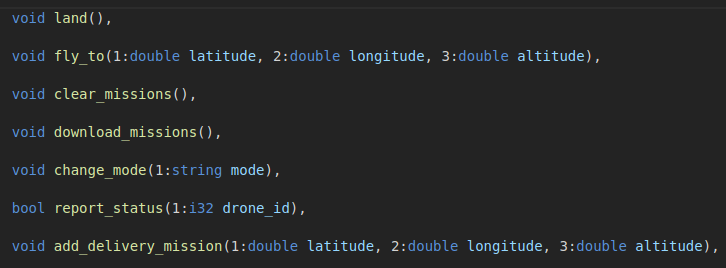
\includegraphics[width=0.9\linewidth, height=5cm]{figures/Ch3/drone_thrift_sample.png} 
%         \caption{Caption1}
%         \label{fig:thrift_service}
%     \end{subfigure}
%     \begin{subfigure}{0.4\textwidth}
%         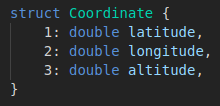
\includegraphics[width=0.9\linewidth, height=5cm]{figures/Ch3/thrift_struct.png}
%         \caption{Caption 2}
%         \label{fig:thrift_struct}
%     \end{subfigure}
% \caption{Caption for this figure with two images}
% \label{fig:thrift}
% \end{figure}

\subsection{Drone Flight Logs}\label{subsect:flightstatus}
Users of the web application supported by this system have the ability to track the position of each drone registered with the app. To accomplish this, the Thrift server running on the Raspberry Pi aboard the drone periodically sends flight logs detailing the altitude, GPS coordinates, and other flight data every 3 seconds to the web application.

This is brought about by sending an HTTP POST request to the REST API endpoint exposed by the web application for the nav logs. The API then inserts an entry in the database with the corresponding data, therefore creating a “log” of the drone\textquotesingle s position. The data is in JSON format, one of the most common microservice data formats.

A sample flight log entry is shown below:
\begin{verbatim}
    nav_log = {
            "gps_latitude": 14.079357,
            "gps_longitude": 100.609541, # AIT Football Field
            "altitude": 20, # in metres
            "battery_voltage": 11.7, # in volts
            "battery_level": 87, # in percentage
            "battery_current": 6.56, # in amperes
            "ekf_ok": true,
            "is_armable": true,
            "system_status": "ACTIVE",
            "mode": "AUTO",
            "armed": true,
            "drone_id": 1,
    }
\end{verbatim}[]

% \begin{figure}[h]
% 	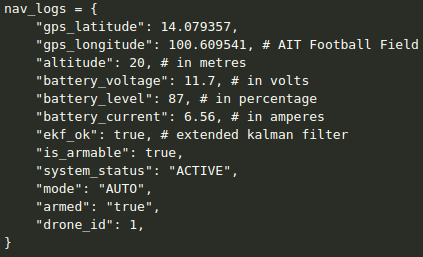
\includegraphics[width=\textwidth]{figures/Ch3/sample_nav_new.png}
% 	\caption{Sample flight log data in JSON.}
% 	\label{fig:json_log}
% \end{figure}
% \FloatBarrier

In addition to the GPS location and altitude of the drone, its current battery level, voltage being supplied to the power module and amperage flowing through the power module, is also included in the JSON message. Evidently, this data depends on the power module working as intended and any fault will result in erroneous values.

The flight logs also detail the mode in which the drone is and whether the drone is armable and armed. This, in conjunction with the battery data, allows for evaluation of the drone's airworthiness and whether the drone needs hardware calibration/maintenance.

Furthermore, in case of a connection loss, the Pixhawk also writes the flight data to an SD card on it in the form of MAVLink log files creating a “black box” of sorts. This will prove helpful in the case of a crash and once the wreckage is recovered. The logged data is comprehensive and its analysis is not covered in this study.

% \subsection{Pixhawk Connection}\label{subsect:pixhawkconnection}
% The Thrift server is connected to the Pixhawk through a UDP wifi connection, provided by a 2.4 GHZ Wifi module that is attached to the Pixhawk by one of the telemetry ports. This means that the Pi doesn't have to connect via wire through these telemetry ports too. For this reason, however, the Pi must remain connected to the Wifi network set up by the Wifi module.

% \subsection{Error Feedback}\label{subsect:pixhawkconnection}
% The Thrift server is connected to the Pixhawk through a UDP wifi connection, provided by a 2.4 GHZ Wifi module that is attached to the Pixhawk by one of the telemetry ports. This means that the Pi doesn't have to connect via wire through these telemetry ports too. For this reason, however, the Pi must remain connected to the Wifi network set up by the Wifi module.

\section{Command Layer}\label{sect:commandlayer}
The Thrift server running on the Raspberry Pi employs the Dronekit API to communicate with the Pixhawk through the MAVLink protocol (see Section \ref{sect:mavlink}). In summary, the Thrift server uploads waypoints created with the mission parameters that the client script has sent from the web server. It then sends the drone on its way. The complete flow diagram of this process for a delivery mission is shown in Figure \ref{fig:commandworkflow}.

The Pixhawk flight controller has several modes in which it can fly the drone. The main flight mode used in the implementation of the system in this study is ``\textbf{AUTO}''. In this ``\textbf{AUTO}'' mode, the Pixhawk simply follows the waypoints and commands uploaded on to it by a GCS in the order in which they were uploaded.

\begin{figure}[t]
	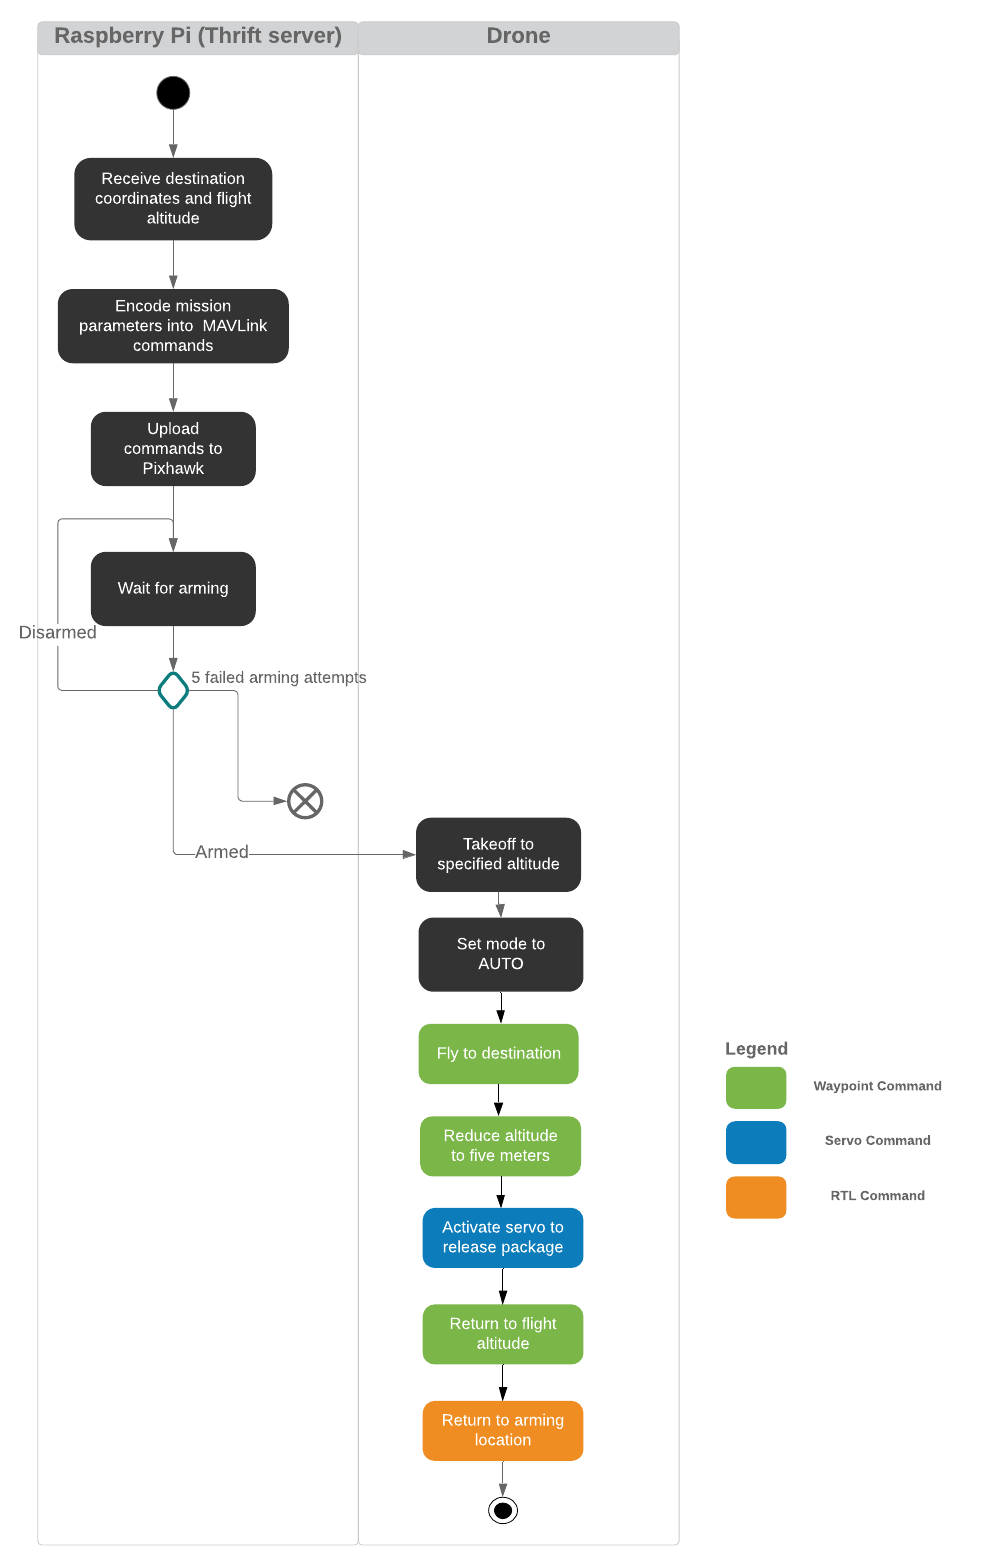
\includegraphics[width=\textwidth, height=21cm]{figures/Ch3/MAVlink_swimlane.png}
	\caption{Complete workflow of command layer for a delivery mission.}
	\label{fig:commandworkflow}
\end{figure}
\FloatBarrier

\begin{table}[t]
 \caption{MAVLink commands used in the implementation.}
 \linespread{0.7}\selectfont
 \begin{center}
     \begin{tabular}{|p{7cm}|p{8cm}|} 
     \hline
     \textbf{MAVLink Commands} & \textbf{Description}\\ 
     \hline
     MAV\_CMD\_NAV\_WAYPOINT & Navigate to waypoint. The latitude, longitude and altitude are specified in the command's parameters.\\
     \hline
     MAV\_CMD\_DO\_SET\_SERVO & Change a servo's PWM value. The servo component's ID and the value itself are specified in the parameters.\\
     \hline
     MAV\_CMD\_NAV\_RETURN\_TO\_LAND & Returns the drone to location where it was armed.\\
     \hline
     \end{tabular}
  \end{center}
 \label{table:mavlinkcmds}
\end{table}
\FloatBarrier

The specific commands used in the Dronekit implementation are shown in Table \ref{table:mavlinkcmds}. These commands are instantiated using the \texttt{Command} Python object, and the MAVLink parameters can also be defined with this object's arguments. An example is shown below.

\begin{verbatim}
    cmd1 = Command(0,0,0,
        mavutil.mavlink.MAV_FRAME_GLOBAL_RELATIVE_ALT,
        mavutil.mavlink.MAV_CMD_NAV_WAYPOINT, 
        0, 0, 0, 0, 0, 0, dest_latitude, dest_longitude, alt
    )
\end{verbatim}[]

As depicted in Figure \ref{fig:waypoint} in Section \ref{subsect:mavlinkcommands}, the last three parameters are used to specify the latitude, longitude and altitude of the waypoint itself. In the case above, the variables \texttt{dest\_latitude}, \texttt{dest\_longitude}, and \texttt{alt} respectively are passed in as parameters for the \texttt{Command}. The exact command is directly imported from the \texttt{pymavlink} library generated from the raw MAVLink library. Other raw MAVLink messages and commands can also be sent using the message encoder provided by Dronekit. For instance, a message to reset the servo on startup is shown below.

\begin{verbatim}
    msg = self.vehicle.message_factory.command_long_encode(
            0, 0,
            mavutil.mavlink.MAV_CMD_DO_SET_SERVO, #command
            0, 
            5,          # param 1 - servo ID
            1900,       # param 2 - desired PWM value
            0,          
            0, 
            0, 0, 0
    )
\end{verbatim}[]

% TODO
% connects with wifi
% \subsection{MAVLink Messages}

% This section will detail the important MAVLink messages in use in this system. There are three main types of commands - navigation, conditional and do (DO). Out of these, the most important are the navigation commands. DO commands are used to control auxiliary devices, not the drone and conditional commands affect only DO commands.

% Navigation commands can be used to control every aspect of the drone’s movements. The most useful of the NAV commands will probably be "MAV\_CMD\_NAV\_WAYPOINT". This simply asks the drone to navigate to the specified location. The location is specified as parameters in the message. This NAV command has seven message parameters and the last three are the target latitude, longitude and altitude that the drone has to follow. Other commands include "MAV\_CMD\_NAV\_TAKEOFF" and "MAV\_CMD\_NAV\_LAND".

\newpage
\section{Limitations}\label{sect:limit}
\subsection{Drone Collision Avoidance}
Due to a lack of a collision avoidance program on the on-board computer, the drone is unable to avoid objects in flight or make adjustments to its speed and altitude. 

This can be remedied by implementing a program that processes the images from a camera, detects objects, and adjusts the drone\textquotesingle's flight accordingly. 

However, for our experiments, the drone follows a clear route without any pedestrian traffic, trees or other obstacles. This implies that the drone will have to fly at a height that would be totally clear of any obstacles (40 metres or higher). 

\subsection{Concurrency}\label{subsect:concurrency}
Currently, the Thrift server is unable to service more than one request at a time, due to the fact that a simple \texttt{TSimpleServer} is used. This implies that multiple mission request will have undesirable effects on the drone.

However, this issue is somewhat mitigated by the fact that the web application is designed to accept only one mission at a time for each drone.

\subsection{Drone Landing}\label{subsect:dronelanding}
The drones used in this project are intended to be serviced and stored in a base. However, due to a lack of an assisted landing program (also with image processing), the drone has some difficulty in landing directly on the base’s “copter-pad”, since it relies solely on its GPS to do so. The estimated accuracy of this GPS-assisted landing is tested in the experiment to validate this limitation (see Section \ref{sect:experimentaldesign} and Section \ref{sect:landingaccuracy}).

If available, the precision landing being developed at the AIT Vision Lab may be implemented into our drone for smoother and more accurate landings.

\newpage
\section{Experimental Design}\label{sect:experimentaldesign}
To validate this project's objectives, a number of drone flights are performed using the system developed. The test destination location is the northwestern edge of the main football field in AIT and the starting point is the southwestern edge. Mission execution is carried out from the web application and the REST API (for the mobile application), although both work in the same way, i.e. through a Thrift client script. The means of validating each objective is defined below.
% \begin{enumerate}
%   \item Use the MAVLink protocol to communicate commands to the  onboard flight controller (Pixhawk PX4) from the onboard computer (Raspberry Pi).
%   \item Communicate user input to the onboard computer through a web interface and an SSH tunnel.
%   \item Develop a command set onto the Raspberry Pi for the automation of base station opening, drone arming, takeoff, mission execution, status reporting, returning to base, and dynamic reaction to mission parameter change.
% \end{enumerate}

\textbf{Objective 1} is stated as follows.
\begin{quote}
    \textbf{Use the MAVLink protocol to communicate commands to the  onboard flight controller (Pixhawk PX4) from the onboard computer (Raspberry Pi).}
\end{quote}

The Raspberry Pi is connected to the Pixhawk through a serial connection to one of the Pixhawk's two telemetry ports. MAVLink commands are sent to the Pixhawk through this connection, using the Dronekit API.

\textbf{Objective 2} is stated as follows.
\begin{quote}
    \textbf{Communicate user input to the onboard computer through a web interface and an SSH tunnel.}
\end{quote}

The drone flies to the location specified by the user on the web application. The web server communicates with the remote drone through the use of an SSH tunnel.

\textbf{Objective 3} is stated as follows.
\begin{quote}
    \textbf{Develop a command set onto the Raspberry Pi for the automation of base station opening, drone arming, takeoff, mission execution, status reporting, returning to base, and dynamic reaction to mission parameter change.}
\end{quote}

The Thrift server on the Raspberry Pi fully automates all of the drone's flight stages, from arming to landing. The Pi also retrieves the vehicle state attributes and sends it to the web server. However, in its unmodified state, the drone lacks the ability to precisely land in its base (see Section \ref{subsect:dronelanding}). Furthermore, the server is capable of accepting input while on a mission, albeit this is limited to only mission termination (see Section \ref{subsect:concurrency}).

To evaluate the system, the primary parameters selected are total flight time, reliability and landing accuracy. Total flight time measures the time taken from when the drone takes off to when it lands again at is takeoff location. Reliability measures the drone's mission success rate in general, i.e., there are no issues with arming, takeoff and it completes its mission flawlessly. Landing accuracy considers the error margin of the landing location relative to the original takeoff location.

% There are two methods of evaluation. The first is with a simulator that mimicks a drone on the web server. In this case, both the Thrift server and client are located on the same machine or address. The second method consists of testing with a real drone. The drone can only be remotely accessed through the SSH tunnel. The Thrift server is running on the Raspberry Pi aboard the drone whereas the client is executed from the web server. Moreover, the Internet connection provided by the LTE module is inherently unpredictable.

% WIll test only in same area - CSIM

% test status
\FloatBarrier